% Generated by julia/to_tex/cubic_tree_table.sh.
\begin{tabular}{@{}ccccc@{}}
\toprule
\rule{0pt}{3ex}$2p_{45}p_{46}p_{56}$ & $+\,p_{23}p_{36}p_{56}$ & $-\,p_{14}p_{12}p_{45}$ & $+\,p_{26}p_{13}p_{45}$ & $-\,p_{35}p_{12}p_{46}$ \tabularnewline[4pt]
% G2 Grassmannian ray 52 over GF(2), simple drawing
\begingroup
\tikzset{
  g2simple taxa/.style={inner sep=0.17em,outer sep=0pt},
  g2simple line/.style={line width=0.6pt,line cap=round},
  g2simple negative/.style={g2simple line,line cap=butt,dash pattern=on 2.4pt off 1.6pt},
  g2simple length/.style={font=\scriptsize,inner sep=0pt},
}
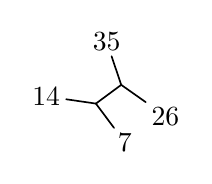
\begin{tikzpicture}[x=1cm,y=1cm,baseline=(current bounding box.center)]
\node[g2simple taxa] (n1) at ({-0.3956cm-0.67em},{0.0594cm+0.1007em}) {14};
\node[g2simple taxa] (n2) at ({0.6472cm+0.67em},{0.0051cm-0.4787em}) {26};
\node[g2simple taxa] (n3) at ({0.1951cm-0.1652em},{0.6171cm+0.495em}) {35};
\node[g2simple taxa] (n4) at ({0.2377cm+0.3657em},{-0.3217cm-0.495em}) {7};
\coordinate (n5) at ({0.0cm+0.0em},{0.0cm+0.0em});
\coordinate (n6) at ({0.3217cm+0.0em},{0.2377cm+0.0em});
\draw[g2simple line] ([shift={(-0.2971pt,0.4022pt)}]n4.126.4547)--([shift={(0.0pt,0.0pt)}]n5);
\draw[g2simple line] ([shift={(0.4944pt,-0.0743pt)}]n1.351.4547)--([shift={(0.0pt,0.0pt)}]n5);
\draw[g2simple line] ([shift={(-0.4068pt,0.2907pt)}]n2.144.4547)--([shift={(0.0pt,0.0pt)}]n6);
\draw[g2simple line] ([shift={(0.1583pt,-0.4743pt)}]n3.288.4547)--([shift={(0.0pt,0.0pt)}]n6);
\draw[g2simple line] ([shift={(0.0pt,0.0pt)}]n5)--([shift={(0.0pt,0.0pt)}]n6);
\end{tikzpicture}
\endgroup
&
% G2 Grassmannian ray 34 over GF(2), simple drawing
\begingroup
\tikzset{
  g2simple taxa/.style={inner sep=0.17em,outer sep=0pt},
  g2simple line/.style={line width=0.6pt,line cap=round},
  g2simple negative/.style={g2simple line,line cap=butt,dash pattern=on 2.4pt off 1.6pt},
  g2simple length/.style={font=\scriptsize,inner sep=0pt},
}
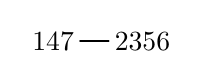
\begin{tikzpicture}[x=1cm,y=1cm,baseline=(current bounding box.center)]
\node[g2simple taxa] (n1) at ({0.0cm+0.0em},{0.0cm+0.0em}) {147};
\node[g2simple taxa] (n2) at ({0.4cm+2.09em},{0.0cm+0.0em}) {2356};
\draw[g2simple line] ([shift={(0.5pt,0.0pt)}]n1.0.0)--([shift={(-0.5pt,0.0pt)}]n2.180.0);
\end{tikzpicture}
\endgroup
&
% G2 Grassmannian ray 9 over GF(2), simple drawing
\begingroup
\tikzset{
  g2simple taxa/.style={inner sep=0.17em,outer sep=0pt},
  g2simple line/.style={line width=0.6pt,line cap=round},
  g2simple negative/.style={g2simple line,line cap=butt,dash pattern=on 2.4pt off 1.6pt},
  g2simple length/.style={font=\scriptsize,inner sep=0pt},
}
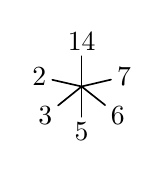
\begin{tikzpicture}[x=1cm,y=1cm,baseline=(current bounding box.center)]
\node[g2simple taxa] (n1) at ({0.0cm-0.0em},{0.4cm+0.495em}) {14};
\node[g2simple taxa] (n2) at ({-0.39cm-0.42em},{0.089cm+0.0959em}) {2};
\node[g2simple taxa] (n3) at ({-0.3127cm-0.42em},{-0.2494cm-0.3349em}) {3};
\node[g2simple taxa] (n4) at ({0.0cm+0.0em},{-0.4cm-0.495em}) {5};
\node[g2simple taxa] (n5) at ({0.3127cm+0.42em},{-0.2494cm-0.3349em}) {6};
\node[g2simple taxa] (n6) at ({0.39cm+0.42em},{0.089cm+0.0959em}) {7};
\coordinate (n7) at ({0.0cm+0.0em},{0.0cm+0.0em});
\draw[g2simple line] ([shift={(0.4875pt,-0.1113pt)}]n2.347.1429)--([shift={(0.0pt,0.0pt)}]n7);
\draw[g2simple line] ([shift={(0.3909pt,0.3117pt)}]n3.38.5714)--([shift={(0.0pt,0.0pt)}]n7);
\draw[g2simple line] ([shift={(0.0pt,0.5pt)}]n4.90.0)--([shift={(0.0pt,0.0pt)}]n7);
\draw[g2simple line] ([shift={(-0.3909pt,0.3117pt)}]n5.141.4286)--([shift={(0.0pt,0.0pt)}]n7);
\draw[g2simple line] ([shift={(-0.4875pt,-0.1113pt)}]n6.192.8571)--([shift={(0.0pt,0.0pt)}]n7);
\draw[g2simple line] ([shift={(0.0pt,-0.5pt)}]n1.270.0)--([shift={(0.0pt,0.0pt)}]n7);
\end{tikzpicture}
\endgroup
&
% G2 Grassmannian ray 40 over GF(2), simple drawing
\begingroup
\tikzset{
  g2simple taxa/.style={inner sep=0.17em,outer sep=0pt},
  g2simple line/.style={line width=0.6pt,line cap=round},
  g2simple negative/.style={g2simple line,line cap=butt,dash pattern=on 2.4pt off 1.6pt},
  g2simple length/.style={font=\scriptsize,inner sep=0pt},
}
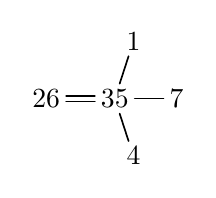
\begin{tikzpicture}[x=1cm,y=1cm,baseline=(current bounding box.center)]
\node[g2simple taxa] (n1) at ({0.1236cm+0.3217em},{0.3804cm+0.99em}) {1};
\node[g2simple taxa] (n2) at ({-0.4cm-1.34em},{0.0cm+0.0em}) {26};
\node[g2simple taxa] (n3) at ({0.0cm+0.0em},{0.0cm+0.0em}) {35};
\node[g2simple taxa] (n4) at ({0.1236cm+0.3217em},{-0.3804cm-0.99em}) {4};
\node[g2simple taxa] (n5) at ({0.4cm+1.09em},{0.0cm-0.0em}) {7};
\draw[g2simple line] ([shift={(-0.1545pt,-0.4755pt)}]n1.252.0)--([shift={(0.1545pt,0.4755pt)}]n3.72.0);
\draw[g2simple line] ([shift={(-0.1545pt,0.4755pt)}]n4.108.0)--([shift={(0.1545pt,-0.4755pt)}]n3.288.0);
\draw[g2simple line] ([shift={(-0.5pt,0.0pt)}]n5.180.0)--([shift={(0.5pt,0.0pt)}]n3.0.0);
\draw[g2simple line] ([shift={(0.5pt,-1.0pt)}]n2.0.0)--([shift={(-0.5pt,-1.0pt)}]n3.180.0);
\draw[g2simple line] ([shift={(0.5pt,1.0pt)}]n2.0.0)--([shift={(-0.5pt,1.0pt)}]n3.180.0);
\end{tikzpicture}
\endgroup
&
% G2 Grassmannian ray 6 over GF(2), simple drawing
\begingroup
\tikzset{
  g2simple taxa/.style={inner sep=0.17em,outer sep=0pt},
  g2simple line/.style={line width=0.6pt,line cap=round},
  g2simple negative/.style={g2simple line,line cap=butt,dash pattern=on 2.4pt off 1.6pt},
  g2simple length/.style={font=\scriptsize,inner sep=0pt},
}
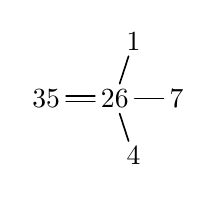
\begin{tikzpicture}[x=1cm,y=1cm,baseline=(current bounding box.center)]
\node[g2simple taxa] (n1) at ({0.1236cm+0.3217em},{0.3804cm+0.99em}) {1};
\node[g2simple taxa] (n2) at ({0.0cm+0.0em},{0.0cm+0.0em}) {26};
\node[g2simple taxa] (n3) at ({-0.4cm-1.34em},{0.0cm+0.0em}) {35};
\node[g2simple taxa] (n4) at ({0.1236cm+0.3217em},{-0.3804cm-0.99em}) {4};
\node[g2simple taxa] (n5) at ({0.4cm+1.09em},{0.0cm-0.0em}) {7};
\draw[g2simple line] ([shift={(-0.1545pt,-0.4755pt)}]n1.252.0)--([shift={(0.1545pt,0.4755pt)}]n2.72.0);
\draw[g2simple line] ([shift={(-0.1545pt,0.4755pt)}]n4.108.0)--([shift={(0.1545pt,-0.4755pt)}]n2.288.0);
\draw[g2simple line] ([shift={(-0.5pt,0.0pt)}]n5.180.0)--([shift={(0.5pt,0.0pt)}]n2.0.0);
\draw[g2simple line] ([shift={(0.5pt,-1.0pt)}]n3.0.0)--([shift={(-0.5pt,-1.0pt)}]n2.180.0);
\draw[g2simple line] ([shift={(0.5pt,1.0pt)}]n3.0.0)--([shift={(-0.5pt,1.0pt)}]n2.180.0);
\end{tikzpicture}
\endgroup
\tabularnewline
\addlinespace[4pt]
\rule{0pt}{3ex}$2p_{23}p_{12}p_{13}$ & $-\,p_{46}p_{14}p_{13}$ & $+\,p_{25}p_{56}p_{23}$ & $+\,p_{16}p_{45}p_{23}$ & $-\,p_{34}p_{56}p_{12}$ \tabularnewline[4pt]
% G2 Grassmannian ray 54 over GF(2), simple drawing
\begingroup
\tikzset{
  g2simple taxa/.style={inner sep=0.17em,outer sep=0pt},
  g2simple line/.style={line width=0.6pt,line cap=round},
  g2simple negative/.style={g2simple line,line cap=butt,dash pattern=on 2.4pt off 1.6pt},
  g2simple length/.style={font=\scriptsize,inner sep=0pt},
}
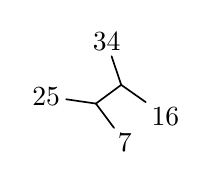
\begin{tikzpicture}[x=1cm,y=1cm,baseline=(current bounding box.center)]
\node[g2simple taxa] (n1) at ({0.6472cm+0.67em},{0.0051cm-0.4787em}) {16};
\node[g2simple taxa] (n2) at ({-0.3956cm-0.67em},{0.0594cm+0.1007em}) {25};
\node[g2simple taxa] (n3) at ({0.1951cm-0.1652em},{0.6171cm+0.495em}) {34};
\node[g2simple taxa] (n4) at ({0.2377cm+0.3657em},{-0.3217cm-0.495em}) {7};
\coordinate (n5) at ({0.0cm+0.0em},{0.0cm+0.0em});
\coordinate (n6) at ({0.3217cm+0.0em},{0.2377cm+0.0em});
\draw[g2simple line] ([shift={(-0.2971pt,0.4022pt)}]n4.126.4547)--([shift={(0.0pt,0.0pt)}]n5);
\draw[g2simple line] ([shift={(0.4944pt,-0.0743pt)}]n2.351.4547)--([shift={(0.0pt,0.0pt)}]n5);
\draw[g2simple line] ([shift={(-0.4068pt,0.2907pt)}]n1.144.4547)--([shift={(0.0pt,0.0pt)}]n6);
\draw[g2simple line] ([shift={(0.1583pt,-0.4743pt)}]n3.288.4547)--([shift={(0.0pt,0.0pt)}]n6);
\draw[g2simple line] ([shift={(0.0pt,0.0pt)}]n5)--([shift={(0.0pt,0.0pt)}]n6);
\end{tikzpicture}
\endgroup
&
% G2 Grassmannian ray 33 over GF(2), simple drawing
\begingroup
\tikzset{
  g2simple taxa/.style={inner sep=0.17em,outer sep=0pt},
  g2simple line/.style={line width=0.6pt,line cap=round},
  g2simple negative/.style={g2simple line,line cap=butt,dash pattern=on 2.4pt off 1.6pt},
  g2simple length/.style={font=\scriptsize,inner sep=0pt},
}
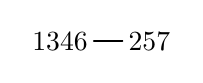
\begin{tikzpicture}[x=1cm,y=1cm,baseline=(current bounding box.center)]
\node[g2simple taxa] (n1) at ({0.0cm+0.0em},{0.0cm+0.0em}) {1346};
\node[g2simple taxa] (n2) at ({0.4cm+2.09em},{0.0cm+0.0em}) {257};
\draw[g2simple line] ([shift={(-0.5pt,0.0pt)}]n2.180.0)--([shift={(0.5pt,0.0pt)}]n1.0.0);
\end{tikzpicture}
\endgroup
&
% G2 Grassmannian ray 10 over GF(2), simple drawing
\begingroup
\tikzset{
  g2simple taxa/.style={inner sep=0.17em,outer sep=0pt},
  g2simple line/.style={line width=0.6pt,line cap=round},
  g2simple negative/.style={g2simple line,line cap=butt,dash pattern=on 2.4pt off 1.6pt},
  g2simple length/.style={font=\scriptsize,inner sep=0pt},
}
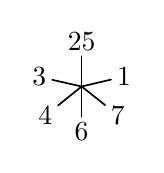
\begin{tikzpicture}[x=1cm,y=1cm,baseline=(current bounding box.center)]
\node[g2simple taxa] (n1) at ({0.39cm+0.42em},{0.089cm+0.0959em}) {1};
\node[g2simple taxa] (n2) at ({0.0cm-0.0em},{0.4cm+0.495em}) {25};
\node[g2simple taxa] (n3) at ({-0.39cm-0.42em},{0.089cm+0.0959em}) {3};
\node[g2simple taxa] (n4) at ({-0.3127cm-0.42em},{-0.2494cm-0.3349em}) {4};
\node[g2simple taxa] (n5) at ({0.0cm-0.0em},{-0.4cm-0.495em}) {6};
\node[g2simple taxa] (n6) at ({0.3127cm+0.42em},{-0.2494cm-0.3349em}) {7};
\coordinate (n7) at ({0.0cm+0.0em},{0.0cm+0.0em});
\draw[g2simple line] ([shift={(-0.4875pt,-0.1113pt)}]n1.192.8571)--([shift={(0.0pt,0.0pt)}]n7);
\draw[g2simple line] ([shift={(0.4875pt,-0.1113pt)}]n3.347.1429)--([shift={(0.0pt,0.0pt)}]n7);
\draw[g2simple line] ([shift={(0.3909pt,0.3117pt)}]n4.38.5714)--([shift={(0.0pt,0.0pt)}]n7);
\draw[g2simple line] ([shift={(0.0pt,0.5pt)}]n5.90.0)--([shift={(0.0pt,0.0pt)}]n7);
\draw[g2simple line] ([shift={(-0.3909pt,0.3117pt)}]n6.141.4286)--([shift={(0.0pt,0.0pt)}]n7);
\draw[g2simple line] ([shift={(0.0pt,-0.5pt)}]n2.270.0)--([shift={(0.0pt,0.0pt)}]n7);
\end{tikzpicture}
\endgroup
&
% G2 Grassmannian ray 41 over GF(2), simple drawing
\begingroup
\tikzset{
  g2simple taxa/.style={inner sep=0.17em,outer sep=0pt},
  g2simple line/.style={line width=0.6pt,line cap=round},
  g2simple negative/.style={g2simple line,line cap=butt,dash pattern=on 2.4pt off 1.6pt},
  g2simple length/.style={font=\scriptsize,inner sep=0pt},
}
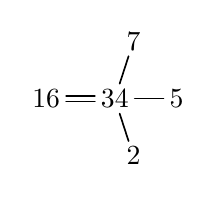
\begin{tikzpicture}[x=1cm,y=1cm,baseline=(current bounding box.center)]
\node[g2simple taxa] (n1) at ({-0.4cm-1.34em},{0.0cm+0.0em}) {16};
\node[g2simple taxa] (n2) at ({0.1236cm+0.3217em},{-0.3804cm-0.99em}) {2};
\node[g2simple taxa] (n3) at ({0.0cm+0.0em},{0.0cm+0.0em}) {34};
\node[g2simple taxa] (n4) at ({0.4cm+1.09em},{0.0cm-0.0em}) {5};
\node[g2simple taxa] (n5) at ({0.1236cm+0.3217em},{0.3804cm+0.99em}) {7};
\draw[g2simple line] ([shift={(-0.1545pt,0.4755pt)}]n2.108.0)--([shift={(0.1545pt,-0.4755pt)}]n3.288.0);
\draw[g2simple line] ([shift={(-0.5pt,0.0pt)}]n4.180.0)--([shift={(0.5pt,0.0pt)}]n3.0.0);
\draw[g2simple line] ([shift={(-0.1545pt,-0.4755pt)}]n5.252.0)--([shift={(0.1545pt,0.4755pt)}]n3.72.0);
\draw[g2simple line] ([shift={(0.5pt,-1.0pt)}]n1.0.0)--([shift={(-0.5pt,-1.0pt)}]n3.180.0);
\draw[g2simple line] ([shift={(0.5pt,1.0pt)}]n1.0.0)--([shift={(-0.5pt,1.0pt)}]n3.180.0);
\end{tikzpicture}
\endgroup
&
% G2 Grassmannian ray 7 over GF(2), simple drawing
\begingroup
\tikzset{
  g2simple taxa/.style={inner sep=0.17em,outer sep=0pt},
  g2simple line/.style={line width=0.6pt,line cap=round},
  g2simple negative/.style={g2simple line,line cap=butt,dash pattern=on 2.4pt off 1.6pt},
  g2simple length/.style={font=\scriptsize,inner sep=0pt},
}
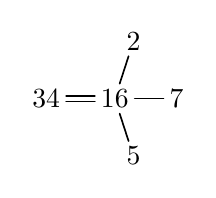
\begin{tikzpicture}[x=1cm,y=1cm,baseline=(current bounding box.center)]
\node[g2simple taxa] (n1) at ({0.0cm+0.0em},{0.0cm+0.0em}) {16};
\node[g2simple taxa] (n2) at ({0.1236cm+0.3217em},{0.3804cm+0.99em}) {2};
\node[g2simple taxa] (n3) at ({-0.4cm-1.34em},{0.0cm+0.0em}) {34};
\node[g2simple taxa] (n4) at ({0.1236cm+0.3217em},{-0.3804cm-0.99em}) {5};
\node[g2simple taxa] (n5) at ({0.4cm+1.09em},{0.0cm-0.0em}) {7};
\draw[g2simple line] ([shift={(-0.1545pt,-0.4755pt)}]n2.252.0)--([shift={(0.1545pt,0.4755pt)}]n1.72.0);
\draw[g2simple line] ([shift={(-0.1545pt,0.4755pt)}]n4.108.0)--([shift={(0.1545pt,-0.4755pt)}]n1.288.0);
\draw[g2simple line] ([shift={(-0.5pt,0.0pt)}]n5.180.0)--([shift={(0.5pt,0.0pt)}]n1.0.0);
\draw[g2simple line] ([shift={(0.5pt,-1.0pt)}]n3.0.0)--([shift={(-0.5pt,-1.0pt)}]n1.180.0);
\draw[g2simple line] ([shift={(0.5pt,1.0pt)}]n3.0.0)--([shift={(-0.5pt,1.0pt)}]n1.180.0);
\end{tikzpicture}
\endgroup
\tabularnewline
\addlinespace[4pt]
\rule{0pt}{3ex}$2p_{46}p_{56}p_{45}$ & $+\,p_{12}p_{25}p_{45}$ & $-\,p_{36}p_{13}p_{46}$ & $+\,p_{15}p_{23}p_{46}$ & $-\,p_{24}p_{13}p_{56}$ \tabularnewline[4pt]
% G2 Grassmannian ray 53 over GF(2), simple drawing
\begingroup
\tikzset{
  g2simple taxa/.style={inner sep=0.17em,outer sep=0pt},
  g2simple line/.style={line width=0.6pt,line cap=round},
  g2simple negative/.style={g2simple line,line cap=butt,dash pattern=on 2.4pt off 1.6pt},
  g2simple length/.style={font=\scriptsize,inner sep=0pt},
}
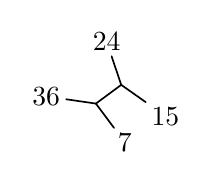
\begin{tikzpicture}[x=1cm,y=1cm,baseline=(current bounding box.center)]
\node[g2simple taxa] (n1) at ({0.6472cm+0.67em},{0.0051cm-0.4787em}) {15};
\node[g2simple taxa] (n2) at ({0.1951cm-0.1652em},{0.6171cm+0.495em}) {24};
\node[g2simple taxa] (n3) at ({-0.3956cm-0.67em},{0.0594cm+0.1007em}) {36};
\node[g2simple taxa] (n4) at ({0.2377cm+0.3657em},{-0.3217cm-0.495em}) {7};
\coordinate (n5) at ({0.0cm+0.0em},{0.0cm+0.0em});
\coordinate (n6) at ({0.3217cm+0.0em},{0.2377cm+0.0em});
\draw[g2simple line] ([shift={(-0.2971pt,0.4022pt)}]n4.126.4547)--([shift={(0.0pt,0.0pt)}]n5);
\draw[g2simple line] ([shift={(0.4944pt,-0.0743pt)}]n3.351.4547)--([shift={(0.0pt,0.0pt)}]n5);
\draw[g2simple line] ([shift={(-0.4068pt,0.2907pt)}]n1.144.4547)--([shift={(0.0pt,0.0pt)}]n6);
\draw[g2simple line] ([shift={(0.1583pt,-0.4743pt)}]n2.288.4547)--([shift={(0.0pt,0.0pt)}]n6);
\draw[g2simple line] ([shift={(0.0pt,0.0pt)}]n5)--([shift={(0.0pt,0.0pt)}]n6);
\end{tikzpicture}
\endgroup
&
% G2 Grassmannian ray 8 over GF(2), simple drawing
\begingroup
\tikzset{
  g2simple taxa/.style={inner sep=0.17em,outer sep=0pt},
  g2simple line/.style={line width=0.6pt,line cap=round},
  g2simple negative/.style={g2simple line,line cap=butt,dash pattern=on 2.4pt off 1.6pt},
  g2simple length/.style={font=\scriptsize,inner sep=0pt},
}
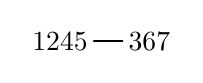
\begin{tikzpicture}[x=1cm,y=1cm,baseline=(current bounding box.center)]
\node[g2simple taxa] (n1) at ({0.0cm+0.0em},{0.0cm+0.0em}) {1245};
\node[g2simple taxa] (n2) at ({0.4cm+2.09em},{0.0cm+0.0em}) {367};
\draw[g2simple line] ([shift={(-0.5pt,0.0pt)}]n2.180.0)--([shift={(0.5pt,0.0pt)}]n1.0.0);
\end{tikzpicture}
\endgroup
&
% G2 Grassmannian ray 30 over GF(2), simple drawing
\begingroup
\tikzset{
  g2simple taxa/.style={inner sep=0.17em,outer sep=0pt},
  g2simple line/.style={line width=0.6pt,line cap=round},
  g2simple negative/.style={g2simple line,line cap=butt,dash pattern=on 2.4pt off 1.6pt},
  g2simple length/.style={font=\scriptsize,inner sep=0pt},
}
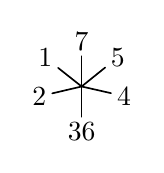
\begin{tikzpicture}[x=1cm,y=1cm,baseline=(current bounding box.center)]
\node[g2simple taxa] (n1) at ({-0.3127cm-0.42em},{0.2494cm+0.3349em}) {1};
\node[g2simple taxa] (n2) at ({-0.39cm-0.42em},{-0.089cm-0.0959em}) {2};
\node[g2simple taxa] (n3) at ({0.0cm-0.0em},{-0.4cm-0.495em}) {36};
\node[g2simple taxa] (n4) at ({0.39cm+0.42em},{-0.089cm-0.0959em}) {4};
\node[g2simple taxa] (n5) at ({0.3127cm+0.42em},{0.2494cm+0.3349em}) {5};
\node[g2simple taxa] (n6) at ({0.0cm+0.0em},{0.4cm+0.495em}) {7};
\coordinate (n7) at ({0.0cm+0.0em},{0.0cm+0.0em});
\draw[g2simple line] ([shift={(0.3909pt,-0.3117pt)}]n1.321.4286)--([shift={(0.0pt,0.0pt)}]n7);
\draw[g2simple line] ([shift={(0.4875pt,0.1113pt)}]n2.12.8571)--([shift={(0.0pt,0.0pt)}]n7);
\draw[g2simple line] ([shift={(-0.4875pt,0.1113pt)}]n4.167.1429)--([shift={(0.0pt,0.0pt)}]n7);
\draw[g2simple line] ([shift={(-0.3909pt,-0.3117pt)}]n5.218.5714)--([shift={(0.0pt,0.0pt)}]n7);
\draw[g2simple line] ([shift={(0.0pt,-0.5pt)}]n6.270.0)--([shift={(0.0pt,0.0pt)}]n7);
\draw[g2simple line] ([shift={(0.0pt,0.5pt)}]n3.90.0)--([shift={(0.0pt,0.0pt)}]n7);
\end{tikzpicture}
\endgroup
&
% G2 Grassmannian ray 12 over GF(2), simple drawing
\begingroup
\tikzset{
  g2simple taxa/.style={inner sep=0.17em,outer sep=0pt},
  g2simple line/.style={line width=0.6pt,line cap=round},
  g2simple negative/.style={g2simple line,line cap=butt,dash pattern=on 2.4pt off 1.6pt},
  g2simple length/.style={font=\scriptsize,inner sep=0pt},
}
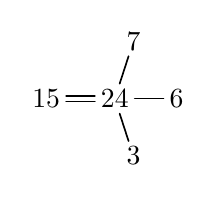
\begin{tikzpicture}[x=1cm,y=1cm,baseline=(current bounding box.center)]
\node[g2simple taxa] (n1) at ({-0.4cm-1.34em},{0.0cm+0.0em}) {15};
\node[g2simple taxa] (n2) at ({0.0cm+0.0em},{0.0cm+0.0em}) {24};
\node[g2simple taxa] (n3) at ({0.1236cm+0.3217em},{-0.3804cm-0.99em}) {3};
\node[g2simple taxa] (n4) at ({0.4cm+1.09em},{0.0cm-0.0em}) {6};
\node[g2simple taxa] (n5) at ({0.1236cm+0.3217em},{0.3804cm+0.99em}) {7};
\draw[g2simple line] ([shift={(-0.1545pt,0.4755pt)}]n3.108.0)--([shift={(0.1545pt,-0.4755pt)}]n2.288.0);
\draw[g2simple line] ([shift={(-0.5pt,0.0pt)}]n4.180.0)--([shift={(0.5pt,0.0pt)}]n2.0.0);
\draw[g2simple line] ([shift={(-0.1545pt,-0.4755pt)}]n5.252.0)--([shift={(0.1545pt,0.4755pt)}]n2.72.0);
\draw[g2simple line] ([shift={(0.5pt,-1.0pt)}]n1.0.0)--([shift={(-0.5pt,-1.0pt)}]n2.180.0);
\draw[g2simple line] ([shift={(0.5pt,1.0pt)}]n1.0.0)--([shift={(-0.5pt,1.0pt)}]n2.180.0);
\end{tikzpicture}
\endgroup
&
% G2 Grassmannian ray 11 over GF(2), simple drawing
\begingroup
\tikzset{
  g2simple taxa/.style={inner sep=0.17em,outer sep=0pt},
  g2simple line/.style={line width=0.6pt,line cap=round},
  g2simple negative/.style={g2simple line,line cap=butt,dash pattern=on 2.4pt off 1.6pt},
  g2simple length/.style={font=\scriptsize,inner sep=0pt},
}
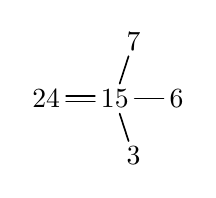
\begin{tikzpicture}[x=1cm,y=1cm,baseline=(current bounding box.center)]
\node[g2simple taxa] (n1) at ({0.0cm+0.0em},{0.0cm+0.0em}) {15};
\node[g2simple taxa] (n2) at ({-0.4cm-1.34em},{0.0cm+0.0em}) {24};
\node[g2simple taxa] (n3) at ({0.1236cm+0.3217em},{-0.3804cm-0.99em}) {3};
\node[g2simple taxa] (n4) at ({0.4cm+1.09em},{0.0cm-0.0em}) {6};
\node[g2simple taxa] (n5) at ({0.1236cm+0.3217em},{0.3804cm+0.99em}) {7};
\draw[g2simple line] ([shift={(-0.1545pt,0.4755pt)}]n3.108.0)--([shift={(0.1545pt,-0.4755pt)}]n1.288.0);
\draw[g2simple line] ([shift={(-0.5pt,0.0pt)}]n4.180.0)--([shift={(0.5pt,0.0pt)}]n1.0.0);
\draw[g2simple line] ([shift={(-0.1545pt,-0.4755pt)}]n5.252.0)--([shift={(0.1545pt,0.4755pt)}]n1.72.0);
\draw[g2simple line] ([shift={(0.5pt,-1.0pt)}]n2.0.0)--([shift={(-0.5pt,-1.0pt)}]n1.180.0);
\draw[g2simple line] ([shift={(0.5pt,1.0pt)}]n2.0.0)--([shift={(-0.5pt,1.0pt)}]n1.180.0);
\end{tikzpicture}
\endgroup
\tabularnewline
\addlinespace[4pt]
\bottomrule
\end{tabular}
